
\section{Casi d'uso}
\subsection{Scopo}

\subsection{Attori}

\subsection{Caricamento dataset}
\begin{figure}[h!]
    \centering
    % Sistema immagine inserendo tag UC e abbelliscila dc
    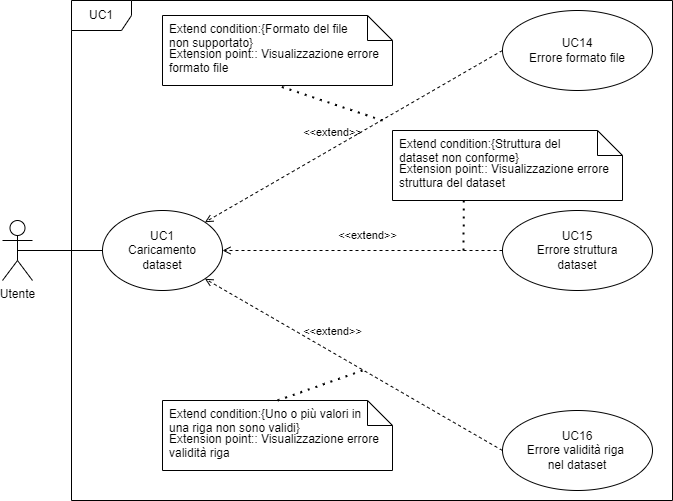
\includegraphics[scale=0.50]{../../assets/Caricamento_dataset.png}
    \caption{UC1 - Caricamento dataset}
\end{figure}
\begin{itemize}
    \item \textbf{Attore primario}: Utente.
    \item \textbf{Precondizioni}: Il sistema è funzionante
    \item \textbf{Postcondizioni}: Viene visualizzato un messaggio che avvisa l'utente del corretto caricamento dei dati e della loro validità. 
                                   I dati vengono caricati nel sistema
    \item \textbf{Scenario principale}:
          \begin{enumerate}
              \item L'utente seleziona il file da caricare
              \item L'utente carica il file
          \end{enumerate}
    \item \textbf{Estensioni}:
    \begin{itemize}
        \item   Nel caso in cui l'utente carichi un file in un formato non supportato
                \begin{enumerate}
                    \item I dati non vengono caricati
                    \item Viene visualizzato un messaggio di errore esplicativo [UC] % To Do: metti il link alla sezione   
                \end{enumerate}
        \item   Nel caso in cui i dati di una o più righe non siano validi
                \begin{enumerate}
                    \item Viene visualizzato un messaggio di errore esplicativo [UC] % To Do: metti il link alla sezione
                \end{enumerate}
    \end{itemize} 
\end{itemize}